\section{Identificación Automática}

\subsection{Descripción del problema}
Según \cite{DC_SPRINGER} la clasificación de texto se define como la asignación de etiquetas a un documento textual basado en su contenido. En este orden de ideas, este aparte del proyecto busca clasificar texto dado que se le van a asignar etiquetas a documentos de un corpus. La tarea de clasificación de texto puede ser entendida como binaria o no binaria, dependiendo de la cardinalidad del conjunto de etiquetas disponibles para la tarea. Un esquema de clasificación binario consta de dos clases únicamente, que suelen ser referidos como una clase positiva o una clase negativa. Por el contrario, un esquema no binario suele contar con más de dos etiquetas.

Dependiendo del esquema usado para la generación del modelo se pueden definir el aprendizaje supervisado y no supervisado. El aprendizaje supervisado consiste en utilizar un conjunto de datos etiquetado para entrenar el modelo. En esta esquema se suelen conocer de antemano las etiquetas a un número de documentos que se usan para el entrenamiento del modelo. En cambio, el aprendizaje no supervisado infiere las características del conjunto de datos de forma automática. En este sentido, no es necesario conocer o haber etiquetado un número de documentos de forma previa. 

A continuación se presentan dos aproximaciones para solucionar el problema de clasificación de texto bajo los esquemas de aprendizaje supervisado y no supervisado. 

\subsection{Revisión del estado del arte}
Antes de resolver el problema de clasificación de texto se procede a realizar la etapa de revisión de literatura. Dentro de la revisión de literatura se encontraron los siguientes artículos relevantes al problema de clasificación de texto:

\begin{itemize}
    \item En \textit{Message passing attention networks for document understanding} \cite{DC_REUTERS} se presenta un modelo de redes de grafos que se evalúa sobre el conjunto de datos de Reuters, entre otros, para su evaluación. Esta aproximación obtuvo un 97.44\% de exactitud sobre el conjunto de datos de \textit{Reuters}. Desafortunadamente este artículo presenta un modelo considerablemente complejo, con redes neuronales desarrolladas específicamente para este propósito y que no son fácilmente accesibles por parte del público. 
    \item En \textit{Transfer learning in biomedical natural language processing: An evaluation of BERT and ELMo on ten benchmarking datasets.} \cite{DC_BERT_ELMO} se presentan los modelos de lenguaje de BERT y ELMo para resolver la tarea de clasificación de documentos relacionados al dominio biomédico. El mejor modelo presentado en el artículo corresponde a un modelo de BERT que fue entrenado exclusivamente sobre documentos biomédicos. Los modelos y el código fuente de este artículo están disponibles para el acceso por parte del público.
    \item En \textit{DocBERT: BERT for Document Classification} \cite{DC_DOCBERT} se presenta un modelo destilado de BERT para la clasificación de documentos. Los autores de este artículo no se enfocan en obtener métricas de evaluación elevadas, sino en simplificar BERT para reducir su tiempo de entrenamiento e inferencia. El resultado final del artículo presenta un modelo destilado de BERT que reduce en treinta veces su cantidad de parámetros. Esta reducción en los parámetros implica que las métricas de evaluación caen en un 3\% como máximo en relación al modelo de BERT original.
    \item Finalmente, en \textit{Text classification with word embedding regularization and soft similarity measure} \cite{DC_REG_EMBEDDING} se presenta un modelo de \textit{embedding}, o vectorización, basado en una regularización. Este artículo sobresale dado que reduce en un 39\% la tasa de error sin utilizar modelos profundos. Sin embargo, el código fuente para la vectorización no está disponible para ser usado por parte del público. 
\end{itemize}

\subsection{Metodología de solución}
A partir de la revisión del estado del arte se pudo establecer que cualquier estrategia de solución debe contar con una serie de pasos estándar. El primer paso consiste en un preprocesamiento de los datos en la que se eliminan las palabras comunes, se eliminan signos de puntuación y se estandarizan y separan las palabras del documento. Debido a que en el preprocesamiento se eliminan palabras claves y se estandarizan las palabras resultantes, este paso es sensible al idioma en el cuál se esté trabajando. \\ 

El segundo paso consiste en calcular la vectorización de los documentos. En este paso se transforma el documento preprocesado en un vector de números reales que lo representa. El cálculo de esta vectorización puede ser realizado mediante diferentes tipos de modelos como lo son BERT, Doc2Vec y otros. Como es de esperar, cada método presenta diferentes valores de desempeño y costo computacional diferentes por lo que deben ser seleccionados dependiendo de las necesidades del usuario. \\

El tercer paso corresponde a la clasificación de las vectorizaciones dependiendo de las necesidades específicas del problema. En este problema en específico es necesario clasificar aquellos documentos que estén relacionados a los siguientes temas:

\begin{itemize}
    \item Vacunas, vacunación y salud mental.
    \item Reapertura de colegios/escuelas y violencia doméstica.
\end{itemize}

Para la clasificación se pueden emplear métodos supervisados y no supervisados dependiendo de los datos que se usen en el entrenamiento. Si bien las vectorizaciones pueden ser iguales para las dos aproximaciones, la diferencia principal radica en el uso de datos etiquetados para los modelos supervisados. A partir de la revisión del estado del arte, se determinó que para la clasificación de texto se  requiere de un mejor modelo de vectorización antes que uno de clasificación. En otras palabras, el buen desempeño de un clasificador de texto suele depender de la vectorización antes del clasificador.

\subsubsection{Preprocesamiento y generación de vectores}
El primer paso de la estrategia de solución consiste en realizar el procesamiento previo de los datos y generar sus respectivos vectores de representación. Para la generación de estos vectores se hace uso de los modelo BERT y Doc2Vec. Cada modelo de vectorización requiere de consideraciones particulares debido a la manera en la cual está configurado su flujo de entrada de datos. El primer modelo, BERT, requiere de un preprocesamiento típico de aplicaciones del procesamiento de lenguaje natural, en el cual se eliminan \textit{stopwords}, signos de puntuación, se realiza el \textit{stemming} de las palabras y se \textit{tokenizan}. Adicionalmente, debido a las limitaciones del modelo BERT sobre el número de \textit{tokens} del documento, es necesario eliminar aquellas palabras que superen el umbral de tokens a partir del inicio del documento. \\

El modelo de Doc2Vec, por su parte, requiere de realizar un preprocesamiento previo que consiste principalmente en convertir el documento en una lista de palabras. Esta lista de palabras se asocia a una etiqueta, la cual corresponde a una cadena de texto con el índice del dato, y que no es relevante para el desarrollo del sistema de clasificación. El modelo de Doc2Vec fue entrenado con la totalidad del corpus de documentos disponibles para cada idioma, salvo por el idioma inglés, con un preprocesamiento diferente para documentos provenientes de redes sociales y de noticias. Debido a la elevada cantidad de documentos disponibles para el idioma inglés, su modelo de Doc2Vec fue entrenado con la mitad de los documentos disponibles. Una vez se ha entrenado el modelo, se proceden a generar las representaciones de los documentos, que corresponden a vectores de 512 posiciones.

\subsubsection{Aproximación no supervisada}
Partiendo de los vectores generados en la etapa anterior, es posible entrenar un modelo de \textit{clustering} para realizar la clasificación no supervisada. En primera instancia, se realiza la selección de modelo: determinar el mejor número de \textit{clusters} para la clasificación. Los modelos de la selección son evaluados con las siguientes tres métricas:

\begin{itemize}
    \item \textbf{Silhouette Score:} es una métrica que permite identificar qué tan cercano se encuentra un dato a la frontera de decisión. La métrica como tal se aplica a cada uno de los datos, pero se puede promediar para obtener una noción sobre la capacidad de clasificación del modelo. La \textit{silhouette score} puede tomar valores entre -1 y +1, donde los valores negativos indican posibles clasificaciones erróneas; los valores cercanos a cero, que se encuentran sobre la frontera de decisión; y, los valores positivos indican una clasificación dentro de un cluster bien definido. 
    \item \textbf{Calinski-Harabasz Index:} es un índice que relaciona la dispersión dentro de los clusters con la dispersión entre los clústers. Este índice tiende a mayores valroes cuando los clusters del modelo son densos y están separados del resto. Este índice puede tomar un valor mínimo de cero, y un valor alto se relaciona con un mejor desempeño del modelo.
    \item \textbf{Davies-Bouldin Index:} es un índice que permite evaluar qué tan similares son los clusters de un modelo. La evaluación se hace mediante la razón entre la distancia entre los centroides de los clusters y el tamaño del cluster. Esta métrica puede tomar un valor mínimo de cero y entre menor sea su valor, se suele asociar a un mejor modelo.
\end{itemize}

\subsubsection{Aproximación supervisada}
De forma similar a la aproximación no supervisada, los modelos supervisados usarán como entrada los vectores generados con los dos modelos presentados previamente. Adicionalmente, dado que se trata de una aproximación supervisada, los datos deberán estar etiquetados. Dentro de esta aproximación se contemplan dos opciones para conocer las etiquetas de los datos. La primera consiste en usar palabras claves presentes en los documentos. Para esta opción se diferencia entre los documentos de noticias y los de redes sociales, ya que los primeros tienen asociados la palabra clave usada en la búsqueda, mientras que los segundos pueden etiquetarse en caso tal que presenten dichas palabras claves. La segunda opción de etiquetado consiste en un etiquetado manual.\\

Teniendo en cuenta el enunciado de los problemas, en los que se deben distinguir documentos de categorías específicas, se propone una solución dentro del esquema de una clasificación binaria. En este sentido, se establece una clase positiva, cuando el documento hace parte de las categorías que se desean identificar, y una clase negativa, cuando el documento no hace parte de estas. Dado que se realiza la clasificación sobre dos conjuntos de categorías, se deben entrenar modelos independientes para cada caso. \\

Los modelos que serán considerados para realizar la clasificación incluyen aproximaciones de aprendizaje profundo, como lo son redes neuronales, y aproximaciones correspondientes a algoritmos como máquinas de vectores de soporte (SVMs, \textit{Support Vector Machines}) o regresiones logísticas, entre otros. En términos generales, lo que se busca con la selección de clasificador es encontrar un modelo capaz de reconocer la información contenida en los vectores con el fin de distinguir si pertenecen a una clase o no.

\subsection{Etiquetado de datos}
Como se mencionó previamente, se utilizan tres estrategias. La primera de ellas es manual, en donde se crea un \textit{script} que permite seleccionar fuente e idioma de los archivos a etiquetar. Este los imprime en pantalla y da el espacio al usuario para indicar un vector de cinco posiciones correspondientes a vacunas, salud mental, reapertura de colegios, violencia intrafamiliar y ninguna de las anteriores. En caso de que se obtenga un archivo que habla de vacunas y reapertura de colegios sería un vector 10100. El código se encarga de operar el vector para almacenarlo en diccionarios.\\

La segunda aproximación consiste en una búsqueda simultánea en múltiples hilos, de una serie de palabras claves para cada uno de los temas en cada uno de los documentos de cada idioma. Se construyen entonces vectores idénticos a los de la primera aproximación y se almacenan en un diccionario cuyas llaves son los nombres de los archivos y los valores un diccionario con las etiquetas de cada clase.\\

La última aproximación toma como base las dos aproximaciones anteriormente mencionadas. Para esto se construyó un modelo de \texttt{doc2vec}, con la librería de \texttt{gensim}, sobre todo el corpus de datos. Con base en esto, se buscaron los documentos más similares (a nivel vectorial) de cada uno de los datos etiquetados manualmente que estuvieran dentro del etiquetado a nivel de palabras clave. De esta manera, se obtiene un \textit{subset} de los datos etiquetados con palabras clave que presenta una similaridad a nivel vectorial con los datos etiquetados manualmente.

\subsection{Resultados}
A continuación se presentan los resultados de las dos aproximaciones contempladas en el desarrollo de este problema:

\subsubsection{Aproximación no supervisada}
La figura \ref{fig:dc_cm_en} presenta la matriz de confusión para la identificación automática de documentos en inglés. Con el fin de facilitar la posible identificación de los \textit{clusters}, se agregan las palabras claves de los documentos usados en la validación. A partir de estas palabras claves, es posible identificar algunos \textit{clusters} de la matriz. El hecho de poder identificar algunos \textit{clusters} no implica que sean clasificados apropiadamente, sino que dicho \textit{clsters} está vinculado estrechamente a aquellos documentos que fueron buscados con la palabra clave. \\

\begin{figure}[H]
    \centering
    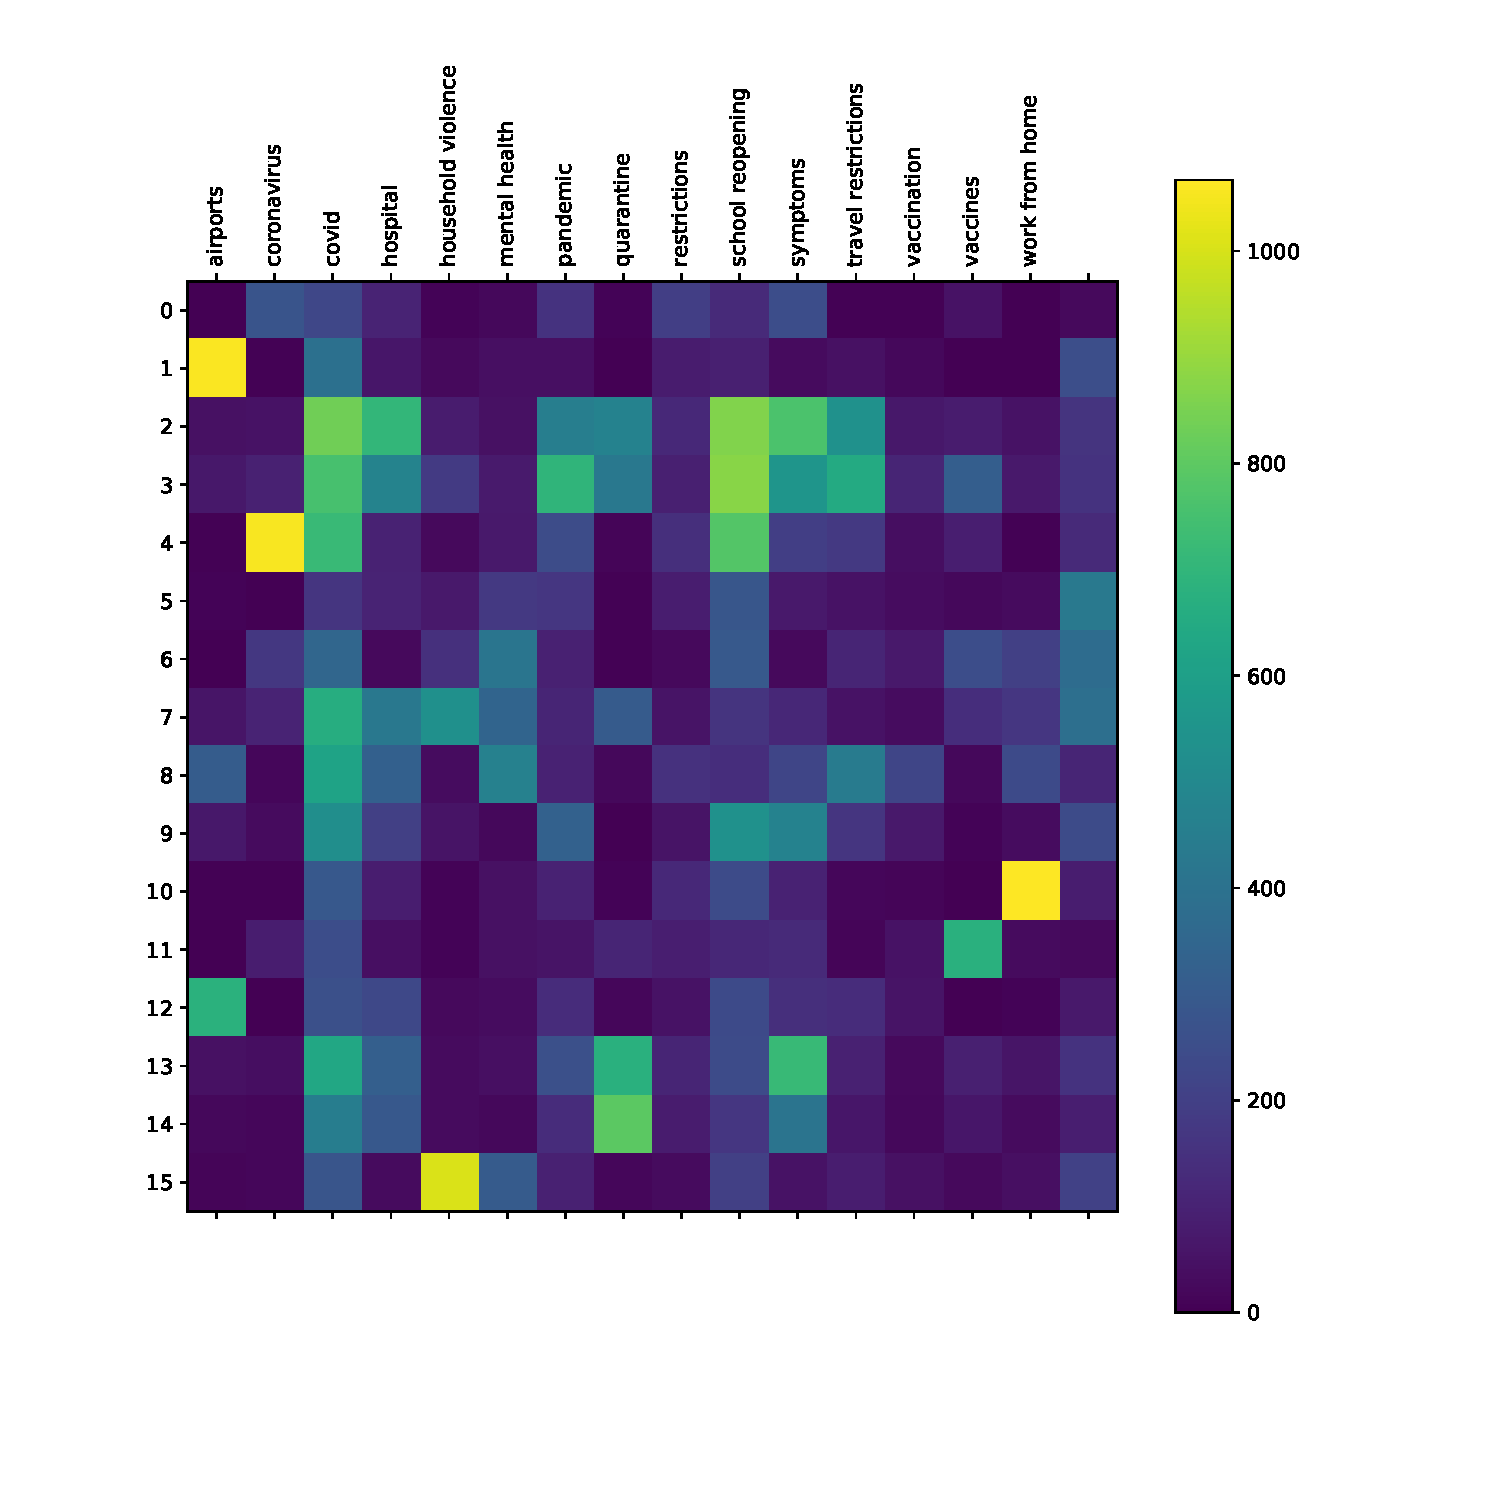
\includegraphics[width=0.75\textwidth]{results/AutomaticIdentification/cf_en.pdf}
    \caption{Matriz de confusión para la clasificación no supervisada de documentos en inglés.}
    \label{fig:dc_cm_en}
\end{figure}

De la figura \ref{fig:dc_cm_en} se puede inferir que términos como \textit{airport}, \textit{coronavirus}, \textit{household violence} y \textit{work from home} están vinculados estrechamente a \textit{clusters} con alta presencia de documentos. Por su parte, términos como \textit{covid}, \textit{hospital}, \textit{pandemic} y \textit{quarentine} no pueden ser asociados a un \textit{cluster} en particular. Una posible explicación a este fenómeno es que estos términos están presentes en la mayoría de los documentos usados en el modelo. Por su parte, la figura \ref{fig:dc_cm_es} presenta la matriz de confusión para la aproximación no supervisada en español. \\

\begin{figure}[H]
    \centering
    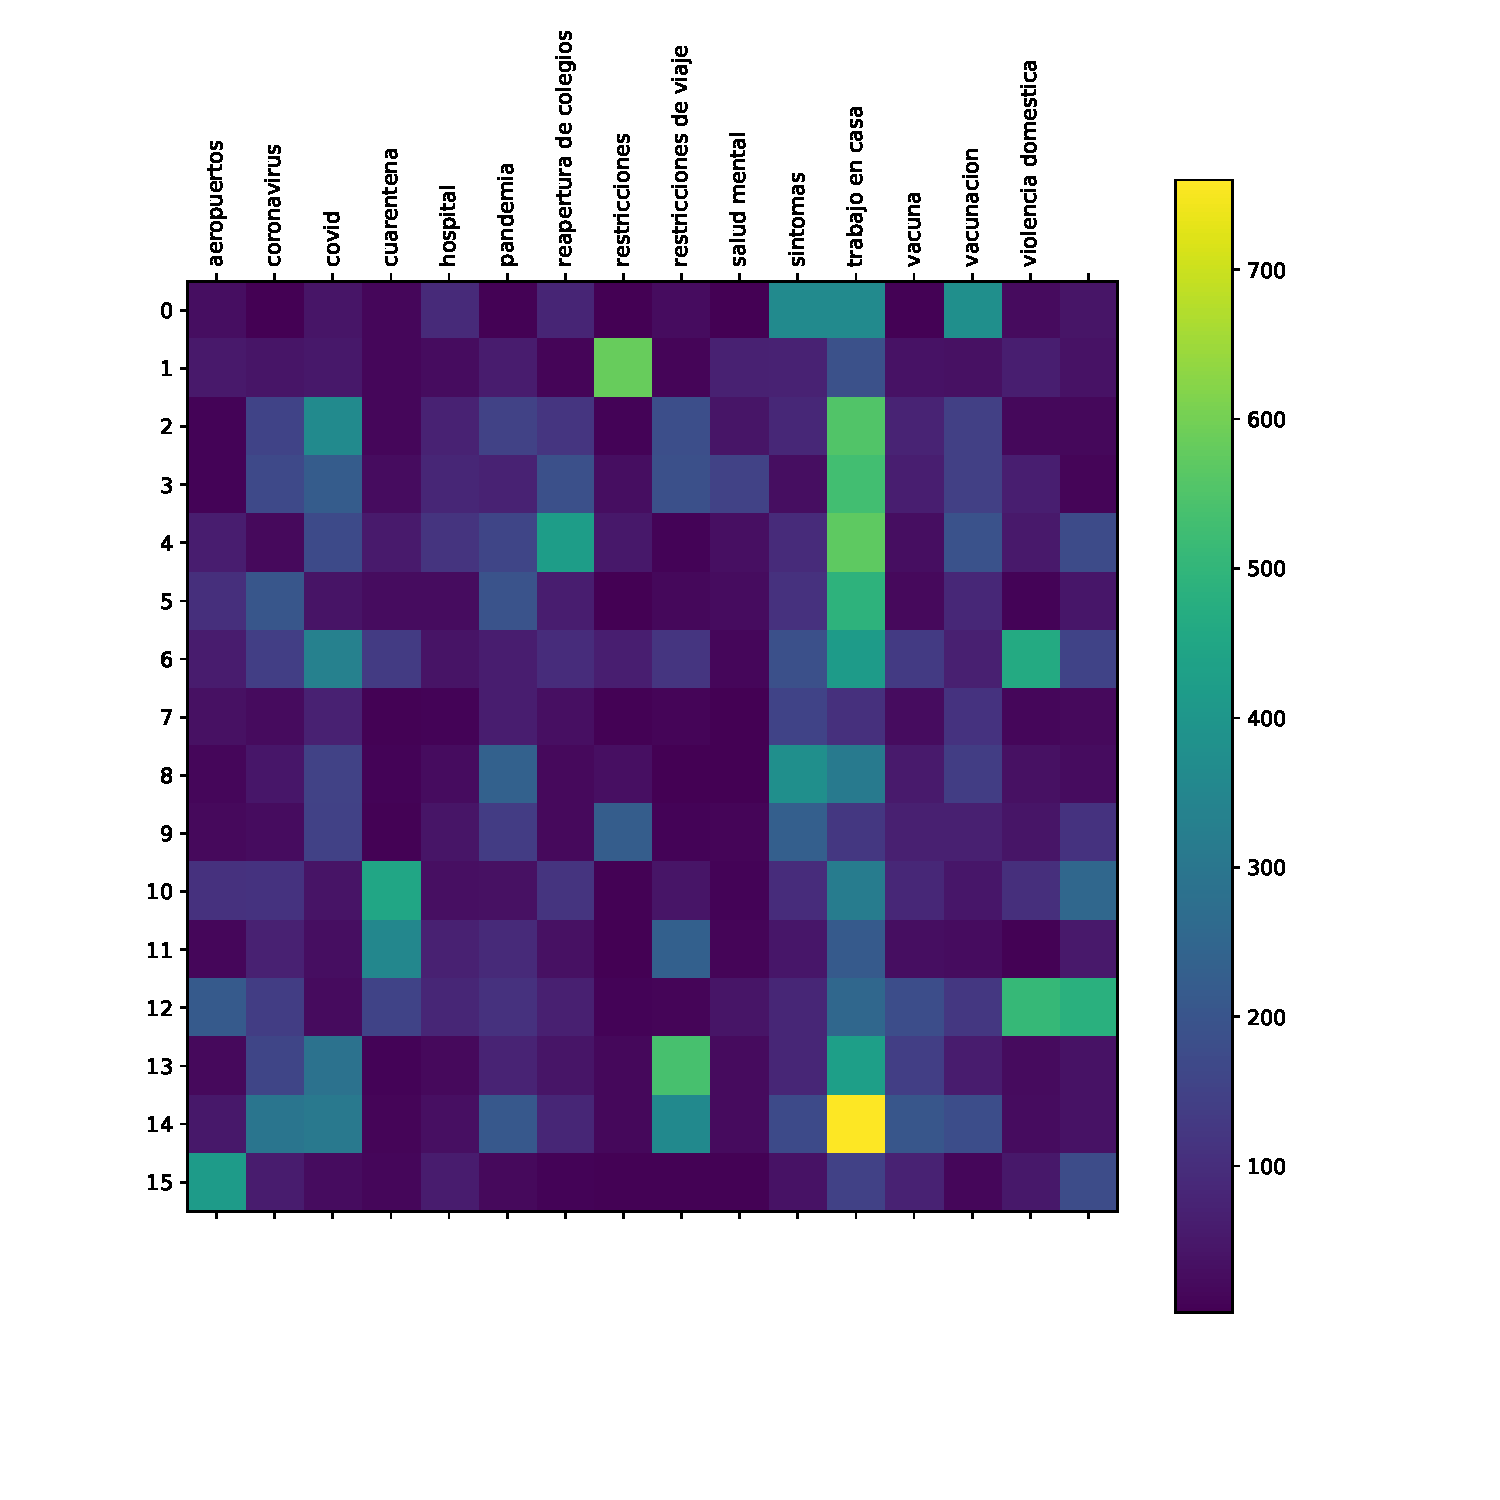
\includegraphics[width=0.75\textwidth]{results/AutomaticIdentification/cf_es.pdf}
    \caption{Matriz de confusión para la clasificación no supervisada de documentos en español.}
    \label{fig:dc_cm_es}
\end{figure}

En la matriz de confusión de la figura \ref{fig:dc_cm_es} se presenta un fenómeno similar a lo ocurrido en la figura \ref{fig:dc_cm_en}: algunos términos pueden ser directamente vinculados a un \textit{cluster} de la matriz, mientras que otros términos no pueden ser vinculados tan estrechamente. Algunos de los términos con una vinculación clara son \textit{aeropuertos}, \textit{reapertura de colegios}, \textit{restricciones}, \textit{vacunación} y \textit{UCI}. Los términos de \textit{cuarentena}, \textit{covid}, \textit{coronavirus} y \textit{trabajo en casa} son los que estaban vinculados a otros \textit{clusters}. Finalmente, la figura \ref{fig:dc_cm_fr} presenta la matriz de confusión asociada al idioma francés. \\

\begin{figure}[H]
    \centering
    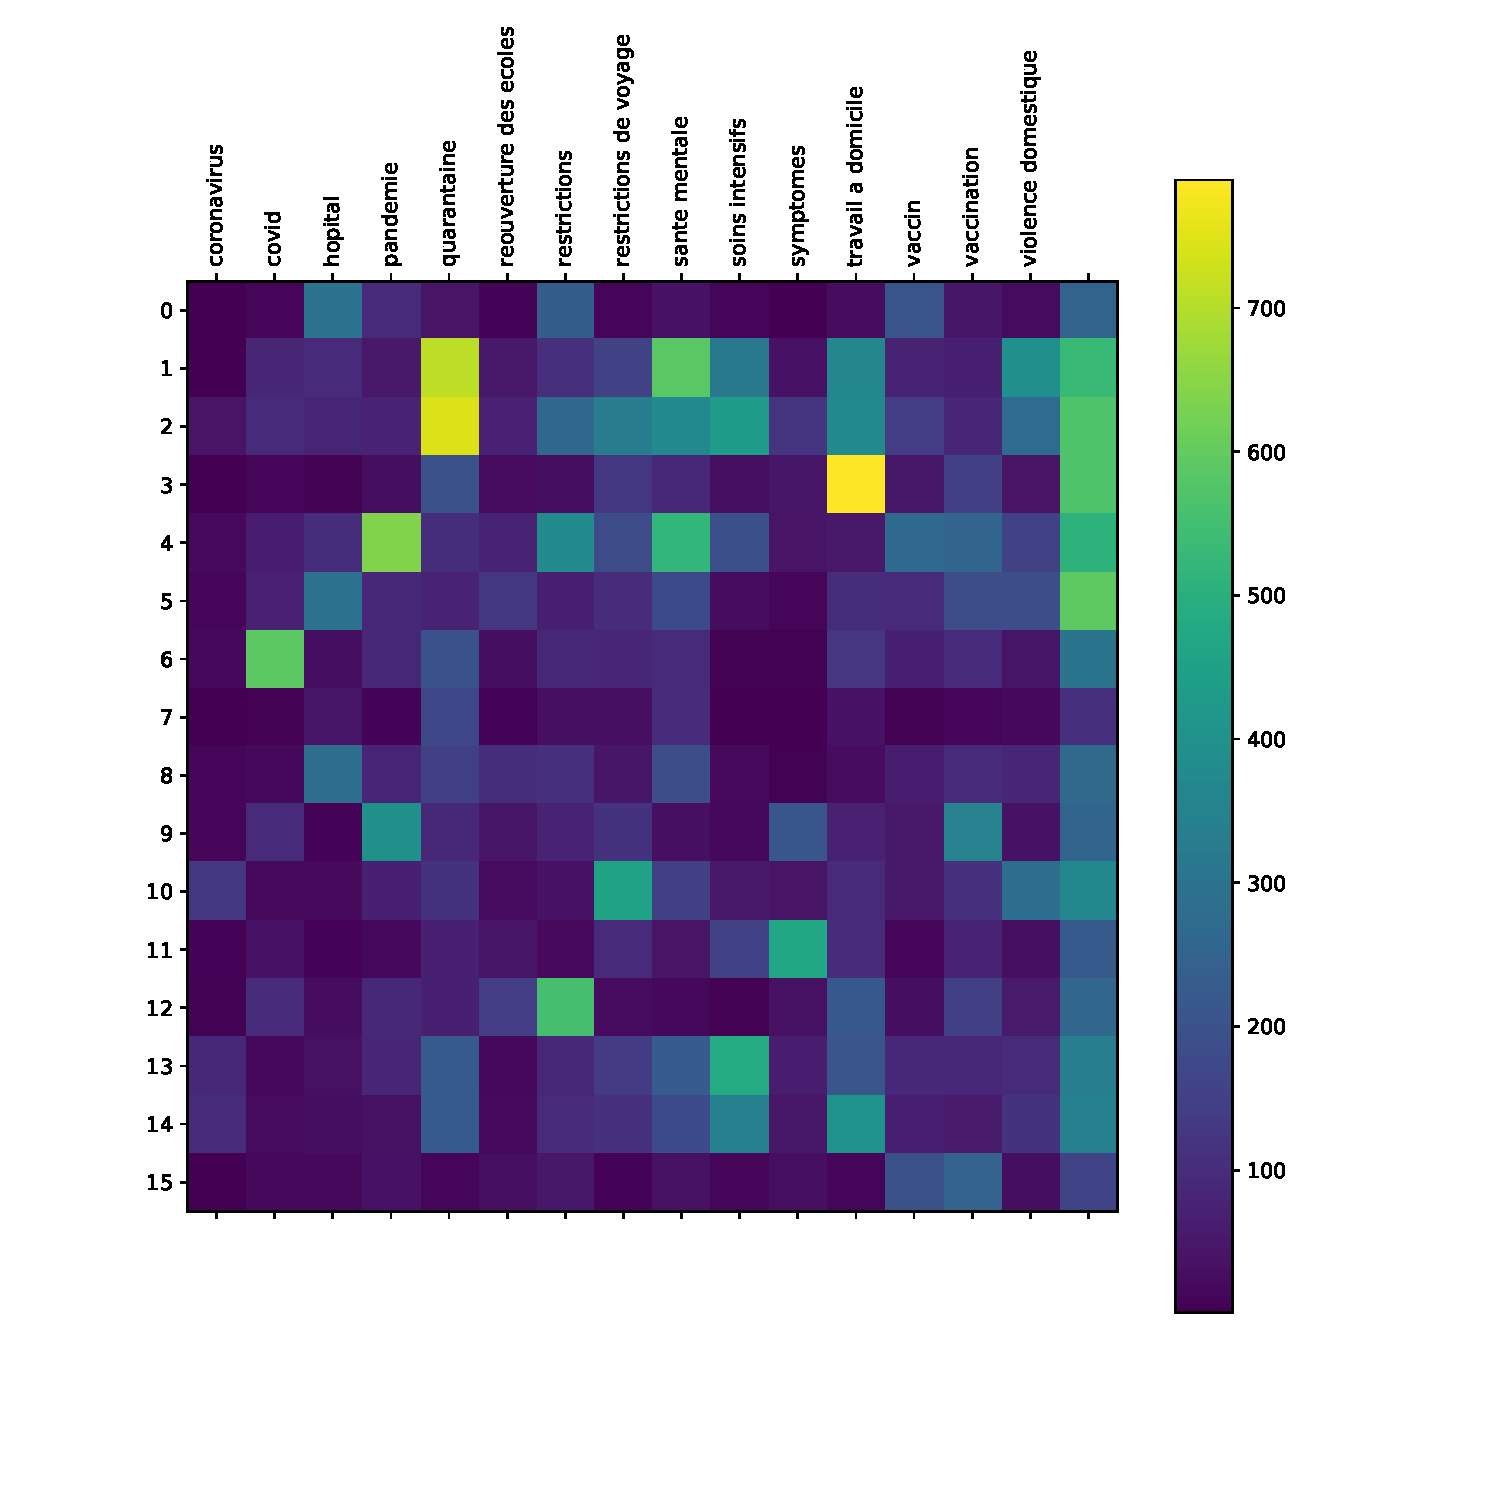
\includegraphics[width=0.75\textwidth]{results/AutomaticIdentification/cf_fr.pdf}
    \caption{Matriz de confusión para la clasificación no supervisada de documentos en francés.}
    \label{fig:dc_cm_fr}
\end{figure}

En la matriz de confusión del idioma francés se presenta un caso diferente a los dos idiomas anteriores. Este caso consiste en que los \textit{clústers} no se pueden asociar tan fácilmente a un solo término, aunque sí se encuentran ciertas correlaciones entre ellos. Por ejemplo, para el \textit{cluster} 1 se tiene la presencia de las palabras \textit{quarantaine} (cuarentena) y \textit{sante mentale} (salud mental). De forma heurística se podrían relacionar los términos dado que se ha evidenciado un aumento en los problemas de salud mental debido a la cuarentena. Sin embargo, vale la pena notar que no es de esperar que el modelo capture esta clase de fenómenos de forma clara. 

\subsubsection{Aproximación supervisada}
La tabla \ref{tab:dc_supervised_metrics_2} presenta los resultados de la red neuronal evaluada para la clasificación sobre aquellos documentos relacionados a vacunas, vacunación y salud mental. Debido a que la clasificación de estos documentos corresponde a un problema no balanceado, se espera que el clasificador tenga un alto nivel de exactitud, como se evidencia en la tabla \ref{tab:dc_supervised_metrics_2}. Sin embargo, las métricas de precisión y \textit{recall} permiten determinar que el modelo es capaz de identificar más de la mitad de los documentos positivos en la clasificación. En las métricas de evaluación se puede interpretar que los resultados están relacionados al número de documentos disponibles para su entrenamiento. Esto se determina dado que el idioma inglés contaba con la mayor cantidad de documentos, seguido de francés y español. Por su parte, la precisión de los modelos sugiere el mismo orden. Un ordenamiento similar sucede con los valores de la métrica de \textit{recall}. 

\begin{table}[H]
    \centering
    \begin{tabular}{|c|c|c|c|}
        \textbf{Idioma} & \textbf{Exactitud} & \textbf{Precisión} & \textbf{Recall} \\ \hline
        Inglés & 86.88\% & 71.34\% & 49.58\% \\
        Español & 84.59\% & 59.22\% & 21.66\%  \\
        Francés & 84.28\% & 66.55\% & 34.53\% \\
    \end{tabular}
    \caption{Resultados de la red neuronal entrenada para la aproximación supervisada en la identificación de vacunas, vacunación y salud mental.}
    \label{tab:dc_supervised_metrics_2}
\end{table}

Por su parte, la tabla \ref{tab:dc_supervised_metrics_3} presenta los resultados de la clasificación sobre documentos relacionados a la apertura de colegios/escuelas y violencia doméstica. En este caso, la cantidad de documentos positivos es menor, por lo que se evidencia una mejora en la métrica de la exactitud. Sin embargo, para la precisión se tiene que el idioma inglés mantiene valores similares al anterior modelo, mientras que los idiomas español y francés reducen su rendimiento. Por parte del \textit{recall} todos los idiomas disminuyeron sus valores, lo cual podría ser explicado por la menor cantidad de datos positivos disponibles para el entrenamiento.

\begin{table}[H]
    \centering
    \begin{tabular}{|c|c|c|c|}
        \textbf{Idioma} & \textbf{Exactitud} & \textbf{Precisión} & \textbf{Recall} \\ \hline
        Inglés & 93.33\% & 71.64\% & 32.41\% \\
        Español & 93.83\% & 57.66\% & 21.26\% \\
        Francés & 92.13\% & 57.32\% & 19.34\% \\
    \end{tabular}
    \caption{Resultados de la red neuronal entrenada para la aproximación supervisada en la identificación de apertura de colegios/escuelas y violencia doméstica.}
    \label{tab:dc_supervised_metrics_3}
\end{table}

\subsection{Conclusiones}
\begin{itemize}
    \item Dentro del dominio de los documentos relacionados a la pandemia del COVID-19 se presentan términos tanto independientes como ampliamente difundidos. Términos como \textit{COVID}, \textit{coronavirus} y \textit{pandemia} aparecen en documentos de distinta índole, haciendo parte de un contexto más que del enfoque principal de los mismos. Por este motivo, términos como \textit{violencia doméstica} y \textit{apertura de colegios} aparecen en menor proporción, lo cuál dificulta su identificación.
    
    \item Se evidenció que es práctica la clasificación de documentos mediante aproximaciones supervisadas y no supervisadas. Aunque la suposición de que la calidad de la clasificación depende principalmente de la vectorización, se pudo corroborar que el modelo utilizado puede influir considerablemente en las métricas de evaluación. La aproximación no supervisada permitió evidenciar que aquellos términos y documentos relacionados a un tema en específico pueden ser identificados directamente. Por otra parte, una aproximación supervisada permite evidenciar el aprendizaje del modelo al contar con métricas mayores a un clasificador aleatorio. 
\end{itemize}
